\begin{defproblem}{funkcie-22}
Zložením ktorých základných elementárnych funkcií vzniknú funkcie dané predpismi
\begin{tasks}(3)
  \task $\sin^3 x$
  \task $\sin (x^3)$
  \task $5^{\tan^2 x}$
  \task $\log_3 \sin^2 \sqrt{b^x}$
  \task $\sqrt{\cos (2^{\sin x})}$
\end{tasks}
\end{defproblem}

\begin{defproblem}{funkcie-23}
Nájdite $D(f)$, ak funkcia $f$ je daná predpisom
\begin{tasks}(2)
  \task $f(x)=\sqrt{3x-x^3}$
  \task $f(x)=\log(x^2-4)$
  \task $f(x)=\sqrt{\sin \sqrt{x}}$
  \task $f(x)=\ln{(\cos (\ln x))}$
  \task $f(x)=\sqrt{\sin 2x}+\sqrt{\sin 3x}$
  \task $f(x)=\sqrt{\cos x^2}$
  \task $f(x)=\sin (\ln \frac{1}{3x+1})$
  \task $f(x)=\ln{(3\sin^2 x -4)}$
  \task $f(x)=\sqrt{9-x^2}+\ln \frac{x+1}{x-2}$
  \task $f(x)=\sqrt{\log \frac{5x-x^2}{4}}$
  \task $f(x)=\log_\frac{1}{2}\log_3 \log_\frac{1}{4} x$
  \task $f(x)=\sqrt{-\sin^2 \zeta x}$
  \task $f(x)=\sqrt[3]{\frac{x+2}{\log\cos x}}$
  \task $f(x)=\sqrt{\log_3 \frac{2x-3}{x-1}}$
  \task $f(x)=\sqrt{\frac{\sin x +\cos x}{\sin x -\cos x}}$
  \task $f(x)=\frac{\sqrt{\cos x -\frac{1}{2}}}{\sqrt{6-35x-6x^2}}$
  \task*(2) $f(x)=\ln{(1-\log (x^2-5x+16))}$
\end{tasks}
\end{defproblem}

\begin{defproblem}{funkcie-24}
Napíšte predpis a určte definičný obor funkcií $f \circ f,f \circ g,g \circ f$
a $g \circ g$, ak
\begin{tasks}
  \task
    \makebox[6cm][l]{$f(x) = x^2$ \hfill}
    $g(x) = 2^x$
  \task
    \makebox[6cm][l]{
      $f(x) = \sgn{x} =
        \begin{cases}
          0,  & \text{ak } x = 0 \\
          1,  & \text{ak } x > 0 \\
          -1, & \text{ak } x > 0
        \end{cases}$
      \hfill
    }
    $g(x)=\frac{1}{x}$
  \task
    \makebox[5cm][l]{
      $f(x) =
        \begin{cases}
          0, & \text{ak }  x \leq 0 \\
          x, & \text{ak }  x > 0
        \end{cases}
      $\hfill
    }
    $g(x) =
      \begin{cases}
        0,    & \text{ak }  x < 0 \\
        -x^2, & \text{ak }  x \geq 0
      \end{cases}
    $
  \task
    \makebox[5cm][l]{
      $f(x) =
        \begin{cases}
          x^2, & \text{ak }  x \in \interval{0}{1} \\
          3x,  & \text{ak }  x \notin \interval{0}{1}
        \end{cases}
      $\hfill
    }
    $g(x) =
      \begin{cases}
        2x,     & \text{ak }  x \in \interval{0}{1} \\
        4x - 2, & \text{ak }  x \notin \interval{0}{1}
      \end{cases}
    $
  \task
    \makebox[7cm][l]{
      $f(x) = D(x) =
        \begin{cases}
          0, & \text{ak }  x \in \mathbb{R} \setminus \mathbb{Q} \\
          1, & \text{ak }  x \in \mathbb{Q}
        \end{cases}$
      \hfill
    }
    $g(x) = \frac{1}{x^2}$
  \task
    \makebox[5cm][l]{
      $f(x) =
        \begin{cases}
          0, & \text{ak }  |x| \leq 1 \\
          1, & \text{ak }  |x| > 1
        \end{cases}$
      \hfill
    }
    $g(x) =
      \begin{cases}
        x^2 - 2, & \text{ak }  |x| \leq 2 \\
        -1,      & \text{ak }  |x| > 2
      \end{cases}$
\end{tasks}
\end{defproblem}

\begin{defproblem}{funkcie-25}
Nech je daná funkcia $f$; označme $f_1:=f,f_2:=f\circ f_1,f_{n+1}:=f\circ f_n$. Nájdite predpis pre $f_n$, ak
\begin{tasks}(2)
  \task $f(x)=\frac{x}{\sqrt{1+x^2}}$;
  \task $f(x)=a+bx$;
  \task $f(x)=\frac{x}{ax+b},(b\neq 1)$.
\end{tasks}
\end{defproblem}

\begin{defproblem}{funkcie-26}
\begin{samepage}
Zistite, či sa rovnajú funkcie $f$ a $g$. Ak nie, nájdite najväčšiu množinu
$A\subset\mathbb{R}$, pre ktorú platí $\frac{f}{A}=\frac{g}{A}$.
\begin{tasks}
  \task
    \makebox[5cm][l]{$f(x)=\sqrt{x(x-1)}$ \hfill}
    $g(x) = \sqrt{x} \sqrt{x-1}$
  \task
    \makebox[5cm][l]{$f(x)=\ln{(x^2-4)}$ \hfill}
    $g(x) = \ln{(x-2)} + \ln{(x+2)}$
  \task
    \makebox[5cm][l]{$f(x) = \cot{x}$ \hfill}
    $g(x) = \frac{1}{\tan{x}}$
  \task
    \makebox[5cm][l]{
      $f(x)=
        \ln{
          \left|
            \frac{\sqrt{x^2 + 1} - x}{\sqrt{x^2 + 1} + x}
          \right|
        }
      $
      \hfill
    }
    $g(x) = -2 \ln{|x+\sqrt{x^2+1}|}$
  \task
    \makebox[6cm][l]{$f(x)=\sqrt{x^2 + 4x + 4} - \sqrt{x^2 - 8x + 16}$ \hfill}
    \\
    $g(x) =
      \begin{cases}
        -6,     & \text{ak } x < -2 \\
        2x - 2, & \text{ak } x \in \interval{-2}{4} \\
        6,      & \text{ak } x > 4
      \end{cases}
    $
\end{tasks}
\end{samepage}
\end{defproblem}

\begin{defproblem}{funkcie-27}
\begin{samepage}
Zostrojte grafy nasledujúcich funkcií:
\begin{tasks}(2)
  \task $y=\ln (1+x)$
  \task $y=1+e^{-x}$
  \task $y=\sin \frac{x}{2}$
  \task $y=3+2\cos 3x$
  \task $y=x^2+4x+2$
  \task $y=\frac{x^2}{2}+x+1$
  \task $y=\frac{1+x}{1-x}$
  \task $y=\frac{2+3x}{1-4x}$
  \task $y=-\sqrt{-x-2}$
  \task $y=\sin 2(x+3)$
  \task $y=\sin (2x+3)$
  \task $y=\frac{1}{3}2^{1-3x}+2$
  \task $y=\tan (2x-\frac{\pi}{2})$
  \task $y=3-0,5\sqrt[3]{3x-2}$
  \task $y=\log_3 (0,5x+2)$
\end{tasks}
\end{samepage}

\begin{solution}
  \textbf{j)}
  Najprv zostrojíme graf funkcie $f(x)=\sin x$, vydelením každej $x$-ovej
  súradnice číslom $2$ (teda jeho \enquote{dvojnásobným zhustením}) z neho
  dostaneme graf funkcie
  \[
    f(2x)=g(x)=\sin 2x
  \]
  Naša funkcia $\sin 2(x+3)$ má tvar $g(x+3)$, jej graf teda získame, ak graf
  funkcie $g$ posunieme pozdĺž osi $Ox$ o $3$ jednotky dĺžky doľava.

  (Pri zostrojovaní takýchto grafov sa často chybne zamieňa poradie
  transformácií. Zistime, graf ktorej funkcie by sme dostali pri ich opačnom
  poradí: posunutím grafu funkcie $f(x) = \sin{x}$ o $3$ jednotky dĺžky vľavo
  získame graf funkcie
  \[
    g_1(x) = f(x + 3) = \sin{(x+3)}
  \]
  ak teraz v tomto grafe vydelíme každú $x$-ovú súradnicu číslom $2$, dostaneme
  graf funkcie
  \[
    g_2(x) = g_1)(2x) = \sin{(2x+3)}
  \]
\end{solution}
\end{defproblem}

\begin{defproblem}{funkcie-28}
Zostrojte grafy nasledujúcich funkcií:
\begin{tasks}(2)
  \task $y=\ln |x|$
  \task $y=\sin |x|$
  \task $y=|\sin x|$
  \task $y=|x^2-2x-1|$
  \task $y=2\cos |x-2|+4$
  \task $y=x|x+2|$
  \task $y=x+\sqrt{x^2}$
  \task $y=|\log_{\frac{1}{2}}(|x|-2)|$
  \task $y=2|x-2|-|x+1|+x$
  \task $y=
    \begin{cases}
      \sin x,          & \text{ak } x \in \interval{-\pi}{0} \\
      2,               & \text{ak } x \in \interval[open left]{0}{1} \\
      \frac{1}{(x-1)}, & \text{ak } x \in \interval[open left]{1}{4}
    \end{cases}
  $
\end{tasks}
\end{defproblem}

\begin{defproblem}{funkcie-29}
Nech graf funkcie $g:\mathbb{R}\rightarrow\mathbb{R}$ je symetrický s grafom funkcie $f$
\begin{tasks}(2)
  \task podľa priamky $x=x_0$
  \task podľa priamky $y=y_0$
  \task podľa bodu $(x_0,y_0)$
\end{tasks}
Vyjadrite funkčné hodnoty funkcie $g$ pomocou funkčných hodnôt funkcie $f$!
\end{defproblem}

\begin{defproblem}{funkcie-30}
Načrtnite približne grafy funkcií:
\begin{tasks}(2)
  \task $y=\sin x^2$
  \task $y=\sin \frac{1}{x}$
  \task $y=x\sin x$
  \task $y=e^x\cos x$
  \task $y=\frac{\sin x}{x}$
  \task $y=\frac{\cos x}{1+x^2}$
\end{tasks}

\begin{solution}
  \textbf{c)}
  Pre $x = k \pi, k \in \mathbb{Z}$, je $y = 0$, pre $x = \frac{\pi}{2} +
  2k\pi,k\in\mathbb{Z}$, ležia príslušné body grafu funkcie $y= x \sin{x}$ na
  priamke $y = x$, pre $x = \frac{3\pi}{2} + 2k\pi, k\in\mathbb{Z}$, na priamke
  $y = -x$. Pretože pre $x \geq 0$ je $-x \leq x \sin{x} \leq x$, pre $x < 0$ je
  $x\leq x\sin x\leq -x$, leží graf funkcie $y = x\sin x$ ``medzi'' priamkami $y
  = x$ a $y = -x$. Na základe toho už vieme približne načrtnúť tento obrázok:
  \begin{center}
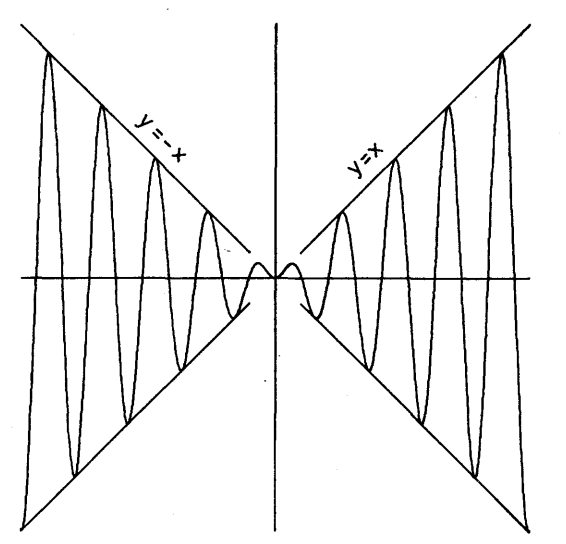
\includegraphics[scale=0.5]{img/pr. 30.png}
\end{center}
\end{solution}
\end{defproblem}

\begin{defproblem}{funkcie-31}
Zostrojte grafy nasledujúcich funkcií tak, že predpis $y=a\cos x +b\sin x$
upravíte na tvar $y=A\sin (x-x_0)$:
\begin{tasks}(2)
  \task $y=\sqrt{3}\cos x +\sin x$
  \task $y=\cos x -\sin x$
  \task $y=6\cos x +8\sin x$
\end{tasks}

\begin{solution}
\textbf{a)}
\vspace{-.5cm}
\begin{align*}
  y
    &= \sqrt{3} \cos{x} + 1 \cdot \sin{x}
      = 2(\frac{\sqrt{3}}{2} \cos{x} + \frac{1}{2}\sin{x}) \\
    &= 2(\sin{\frac{\pi}{3}} \cos{x} + \cos{\frac{\pi}{3}}\sin{x})
      = 2\sin{(x + \frac{\pi}{3})}
\end{align*}
(táto úprava je analogická úprava algebraického tvaru komplexného čísla $a + bi$
na goniometrický tvar $\sqrt{a^2 + b^2}(\cos{\varphi} + i \sin{\varphi)}$).
\end{solution}
\end{defproblem}

\begin{defproblem}{funkcie-32}
Ukážte, že grafy funkcií $f(x)=x^3-3a^2x$ a $g(x)=x^3-3ax^2$ možno získať jeden z druhého posunutím.
\end{defproblem}

\begin{defproblem}{funkcie-33}
Do jedného obrázku nakreslite grafy funkcií $f$ a $g$, ak
\begin{tasks}(2)
  \task
    $ f(x)=\sin x $ \\
    $ g(x)=-\sqrt{1-\cos^2 x} $
  \task
    $ f(x)=\cos x $ \\
    $ g(x)=\frac{1}{\sqrt{1+\tan^2 x}} $
\end{tasks}
\end{defproblem}

\begin{defproblem}{funkcie-34}
Zostrojte graf funkcie $f:\mathbb{R} \rightarrow \mathbb{R}$, ak:
\begin{tasks}
  \task
    $ f(x+1) = 2 \cdot f(x), x \in \mathbb{R} $ \\
    $ f(x) = x(1-x), x \in \interval{0}{1} $
  \task
    $ f(x+\pi)=f(x) + \sin{x}, x \in \mathbb{R} $ \\
    $ f(x) = 0; x \in \interval{0}{\pi} $
\end{tasks}
\end{defproblem}

%aj tu by som dala M do samostatneho stlpca ako je to v skriptach originalnych
\begin{defproblem}{funkcie-35}
Zistite, či funkcia $f$ je na množine $M$ ohraničená zhora, resp. zdola:
\begin{tasks}
  \task
      $f(x) = \sin\frac{1}{x}$,
      $M = \interval[open]{0}{1}$
  \task
    $f(x) = \frac{1}{4+x^2}$,
    $M = \interval[open right]{2}{\infty}$
  \task
    $f(x)=\frac{x+5}{x-1}$,
    $M = \interval[open left]{1}{2}$
\end{tasks}
\end{defproblem}

\begin{defproblem}{funkcie-36}
Pomocou symbolov $\forall,\exists$ zapíšte výrok \enquote{hodnota $f(x_0)$ nie je
maximom funkcie $f$ na množine $B$ $(x_0\in B\subset D(f))$}.
\end{defproblem}

\begin{defproblem}{funkcie-37}
Nech je daná funkcia $f:\mathbb{R}\rightarrow(0,\infty)$. Potom funkcia $g$
určená predpisom $g(x)=\frac{1}{f(x)}$ je ohraničená práve vtedy, keď
$\inf\limits_{x\in\mathbb{R}}f(x)>0$. Dokážte!
\end{defproblem}

\begin{defproblem}{funkcie-38}
Nech funkcie $f$ a $g$, definované na $\mathbb{R}$, sú zhora ohraničené. Potom
\[
  \sup_{x\in\mathbb{R}}(f(x)+g(x))
  \leq
  \sup_{x\in\mathbb{R}} f(x) + \sup_{x\in\mathbb{R}} g(x)
\]
Dokážte!
\end{defproblem}

\begin{defproblem}{funkcie-39}
Uveďte príklad neohraničených funkcií $f$, $g$ definovaných na $\mathbb{R}$,
ktorých superpozícia je ohraničená funkcia!
\end{defproblem}

\begin{defproblem}{funkcie-40}
\par
\needspace{2\baselineskip}
Vyšetrite rast a klesanie funkcií:
\begin{tasks}(2)
  \task $f(x)=\sin x +\cos x$
  \task $f(x)=\sin^4 x +\cos^4 x$
\end{tasks}
\end{defproblem}

\begin{defproblem}{funkcie-41}
Dokážte: Ak postupnosť $\{\frac{a_n}{b_n}\}_{n=1}^\infty$ $(b_n>0$ pre
$n\in\mathbb{N}$) je monotónne, tak aj postupnosť
\[
  \frac{a_1+a_2+...+a_n}{b_1+b_2+...+b_n}\}_{n=1}^\infty
\]
je monotónna.
\end{defproblem}

\begin{defproblem}{funkcie-42}
Pomocou symbolov $\forall,\exists$ zapíšte výroky
\begin{tasks}
\task
  Funkcia $f:\mathbb{R} \rightarrow \mathbb{R}$ nie je klesajúca na množine $M$ \\
  $(\emptyset \neq M\subset\mathbb{R})$
\task
  Funkcia $f:A \rightarrow \mathbb{R}$ nie je monotónna na množine $M$ \\
  $(\emptyset \neq M\subset A \subset\mathbb{R})$
\end{tasks}
\end{defproblem}

\begin{defproblem}{funkcie-43}
\begin{samepage}
Ukážte, že nasledujúce funkcie nie sú monotónne:
\begin{tasks}(2)
  \task $f(x) = x^2 - 3x + 4$
  \task $f(x) = \sgn^2 x$
  \task $f(x) = \tan x$
\end{tasks}
\end{samepage}
\begin{solution}
  \textbf{a)}
  Pre $x=0$ a $y=1$ platí $x<y\wedge f(x)>f(y)$; pre $x=2$ a $y=3$ platí
  $x<y\wedge f(x)<f(y)$. Preto funkcia $f$ nemôže byť nerastúca (a teda nemôže
  byť ani klesajúca), tomu totiž odporuje voľba $x=2,y=3$; súčasne $f$ nemôže
  byť neklesajúca (a teda nemôže byť ani rastúca), tomu odporuje voľba
  $x=0,y=1$. (Samozrejme, že pri výbere vhodných $x,y$ sme si pomáhali grafom
  funkcie $f$.)
  \end{solution}
\end{defproblem}

\begin{defproblem}{funkcie-44}
Uveďte príklad funkcie $f:\mathbb{R} \rightarrow \mathbb{R}$, ktorá je rastúca
na $\interval[open right]{0}{1}$, rastúca na $\interval[open right]{1}{2}$, ale
nie je rastúca na $\interval[open right]{0}{2}$!
\end{defproblem}

\begin{defproblem}{funkcie-45}
Nech funkcie $f,g$ sú klesajúce a záporné na množine $M$. Rozhodnite o
monotónnosti nasledujúcich funkcií na množine $M$ a svoje tvrdenia dokážte:
\begin{tasks}(4)
  \task $f(x) \cdot g(x)$
  \task $f^3(x)$
  \task $f(x) + Bg(x)$
  \task $g^6(x)$
\end{tasks}
\end{defproblem}

\begin{defproblem}{funkcie-46}
\begin{tasks}
\task Dokážte, že superpozícia rýdzomonotónnych funkcií je rýdzomonotónna funkcia!
\task Vyšetrite rast a klesanie funkcií
\begin{enumerate}
  \item $f(x)=\log (x^2-6x+10)$
  \item $f(x)=\log_\frac{1}{2}(x^2-8x+20)$
\end{enumerate}
\end{tasks}
\end{defproblem}

\begin{defproblem}{funkcie-47}
Uveďte príklady funkcií $f,g:\mathbb{R}\rightarrow\mathbb{R}$ takých, že
\begin{tasks}
\task
  $f$ je rastúca, $g$ klesajúca, $f+g$ rastúca
\task
  $f$ je rastúca na $(0,1)$, $g$ klesajúca na $(0,1)$, $f\cdot g$ nie je
  rastúca na $(0,1)$
\end{tasks}
\end{defproblem}

\begin{defproblem}{funkcie-48}
Dokážte, že:
\begin{tasks}
\task každé kladné racionálne číslo je periódou Dirichletovej funkcie
\task žiadne kladné iracionálne číslo nie je jej perodou
\end{tasks}
\end{defproblem}

\begin{defproblem}{funkcie-49}
Ak najmenšou periódou funkcie $f$ je číslo $T$, tak najmenšou periódou funkcie
$g(x):=f(ax+b)$ $(a>0)$ je číslo $\frac{T}{a}$. Dokážte!
\end{defproblem}

\begin{defproblem}{funkcie-50}
Zostrojte graf funkcie $f:\mathbb{R} \rightarrow \mathbb{R}$ s periódou $1$, ak
pre $x \in \interval[open right]{0}{1}$ platí $f(x) = x^2$.
\end{defproblem}

\begin{defproblem}{funkcie-51}
Dokážte: Ak existuje $T>0$ také, že platí niektorá z nasledujúcich podmienok,
tak funkcia $f:\mathbb{R} \rightarrow \mathbb{R}$ je periodická:
\begin{tasks}(2)
  \task $f(x+T)=-f(x),x\in\mathbb{R}$
  \task $f(x+T)=\frac{1}{f(x)},x\in\mathbb{R}$
  \task $f(x+T)=\frac{f(x)+a}{bf(x)-1},x\in\mathbb{R}$
  \task $f(x+T)=\frac{1}{1-f(x)},x\in\mathbb{R}$
\end{tasks}
\end{defproblem}

\begin{defproblem}{funkcie-52}
Ak graf funkcie $f:\mathbb{R} \rightarrow \mathbb{R}$ je symetrický podľa osí
$x = a,x = b$ $(a < b)$, tak $f$ je periodická funkcia. Dokážte!
\end{defproblem}

\begin{defproblem}{funkcie-53}
Zistite, či je daná funkcia prostá; ak áno, nájdite k nej inverznú funkciu a
určte jej definičný obor:
\begin{tasks}(2)
  \task $f(x)=\frac{1-x}{1+x}$
  \task $f(x)=\frac{x}{x^2+2}$
  \task $f(x)=\frac{2x}{1-x^2},x \leq -1$
  \task $f(x)=\frac{2x}{1+x^2},x \in \interval{-1}{1}$
  \task $f(x)=3^{\frac{x}{x-1}}$
  \task $f(x)=2^{x^2-2x},x\leq 1$
  \task $f(x)=\frac{10^x-10^{-x}}{10^x+10^{-x}}+1$
  \task $f(x)=1+\sqrt{3+e^{2x}}$
  \task $f(x)=\log_x 10$
  \task $f(x)=2^{1+\ln\sqrt{x-2}}$
  \task $f(x)=\frac{1}{2}(x-\frac{1}{x}),x>0$
  \task $f(x)=\frac{1}{2}(x-\frac{1}{x}),x<0$
  \task $f(x)=x+\sqrt{x^2-1}$
  \task $f(x)=\log_2 (x+\sqrt{x^2+1})$
  \task
    $f(x)=
      \begin{cases}
        x,  & \text{ak } x < 0 \\
        2x, & \text{ak } x \geq 0
      \end{cases}
    $
  \task
    $f(x)=
      \begin{cases}
        x,  & \text{ak } x < 0 \\
        2x, & \text{ak } x \geq 0
      \end{cases}
    $
  \task
    $f(x)=
      \begin{cases}
        x,   & \text{ak } x \in \mathbb{Q} \\
        1-x, & \text{ak } x \notin \mathbb{Q}
      \end{cases}
    $
  \task
    $f(x)=
      \begin{cases}
        x-1, & \text{ak } x < 1 \\
        x^2, & \text{ak } x \in \interval{1}{4} \\
        2^x, & \text{ak } x > 4
      \end{cases}
    $
\end{tasks}

\begin{solution}
  \textbf{c)}
  Pre každé $x \in \mathbb{R}$ nájdime všetky tie $y \in D(f)$, pre ktoré $f(y)
  = x$, t.j. všetky tie $y \leq -1$, pre ktoré $\frac{2y}{(1-y^2)} = x$. Ak je
  $x$ dané, musia byť hľadané čísla $y$ riešeniami rovnice $$xy^2+2y-x=0;$$
  tejto pre $x=0$ vyhovuje len $y=0$, pre $x\neq 0$ jej vyhovujú čísla
  \[
    y_1=\frac{-1+\sqrt{1+x^2}}{x}, y_2=\frac{-1-\sqrt{1+x^2}}{x}
  \]
  Pretože hľadáme len riešenia ležiace v intervale $\interval[open
  left]{-\infty}{-1}$, musíme zistiť, kedy $y_1\leq -1$ a kedy $y_2\leq -1$.
  Prvá z týchto nerovností nie je splnená pre žiadnu $x\neq 0$, druhá platí pre
  každé $x>0$.

  Zistili sme teda: pre žiadne $x\neq 0$ neexistuje $y\neq -1$ také, že
  $f(y)=x$; pre každé $x>0$ existuje práve jedno číslo $y\leq -1$, pre ktoré
  $f(y)=x$, toto číslo je určené vzťahom:
  \[
    y=-\frac{(1+\sqrt{1+x^2})}{x}
  \]
  To znamená:
  \begin{itemize}
    \item funkcia $f$ je prostá
    \item $f(\interval[open left]{-\infty}{-1})=\interval[open right]{0}{\infty}$
    \item
      inverzná funkcia $f^{-1}$ je definovaná na množine
      $f(\interval[open left]{-\infty}{-1})$ predpisom
      \[
        f^{-1}(x)=-\frac{(1+\sqrt{1+x^2})}{x}
      \]
  \end{itemize}
\end{solution}
\end{defproblem}

\begin{defproblem}{funkcie-54}
Dokážte, že graf funkcie $y=\ln (1-e^x)$ je symetrický podľa priamky $y=x$.
\end{defproblem}

\begin{defproblem}{funkcie-55}
\begin{tasks}
\task
  Uveďte príklad funkcie $f:\mathbb{R}\rightarrow\mathbb{R}$, ktorá je prostá, a
  nie je monotónna na $\mathbb{R}$!
\task
  Uveďte príklad funkcie $f:\mathbb{R}\rightarrow\mathbb{R}$, ktorá je prostá, a
  nie je monotónna na žiadnom intervale $I\subset\mathbb{R}$!
\end{tasks}
\end{defproblem}

\begin{defproblem}{funkcie-56}
Rozhodnite o pravdivosti tohto tvrdenia: \enquote{Ak aspoň jedna z funkcií $f,g$
definovaných na $\mathbb{R}$ nie je prostá, tak funkcia $f\circ g$ nie je
prostá.}!
\end{defproblem}

\begin{defproblem}{funkcie-57}
Vypočítajte:
\begin{tasks}(3)
  \task $\arcsin(\sin \frac{7}{3}\pi)$
  \task $\sin(\arcsin \frac{1}{\sqrt{2}})$
  \task $\arccos(\sin \frac{\pi}{6})$
  \task $\arcsin(\cos \frac{13}{3}\pi)$
  \task $\tan(\arccos\frac{1}{2})$
\end{tasks}
\end{defproblem}

\begin{defproblem}{funkcie-58}
\begin{tasks}
\task
  Pomocou funkcie $\arcsin$ vyjadrite inverznú funkciu k zúženiu funkcie
  $\sin$ na interval
  \begin{enumerate*}
    \item $\interval{\frac{3\pi}{2}}{\frac{5\pi}{2}}$
    \item $\interval{\frac{\pi}{2}}{\frac{3\pi}{2}}$
  \end{enumerate*}
\task
  Zostrojte grafy funkcií

  \begin{enumerate*}
    \item $\sin(\arcsin x)$
    \item $\arcsin(\sin x)$
    \item $\cos(\arccos x)$
  \end{enumerate*}

  \begin{enumerate*}[resume]
    \item $\arccos(\cos x)$
  \end{enumerate*}
\end{tasks}
\end{defproblem}

\begin{defproblem}{funkcie-59}
\begin{samepage}
Nájdite inverznú funkciu k funkcii
\begin{tasks}(2)
  \task $f(x)=\sin^3 x, x \in \interval{-\frac{\pi}{2}}{\frac{\pi}{2}}$
  \task $f(x)=\sin^3 x, x \in \interval{\frac{\pi}{2}}{\frac{3\pi}{2}}$
  \task $f(x)=\sin^2 (\frac{\pi}{2}),x \in \interval{2\pi}{3\pi}$
  \task $f(x)=\arctan\frac{1}{x}$
  \task $f(x)=4\arcsin\sqrt{1-x^3}$
  \task $f(x)=3+4\arccos(2x-1)$
  \task $f(x)=2^{3+\arctan x}$
  \task! $f(x)=\tan{x},
    x \in \interval[open right]{-\pi}{0} \setminus \{-\frac{\pi}{2}\}
  $
  \task*(2) $f(x)=\sin{(3x-1)}, |6x-2| < \pi$
\end{tasks}
\end{samepage}
\end{defproblem}

\begin{defproblem}{funkcie-60}
Dokážte rovnosť funkcií $\sin(\arccos x)$ a $\sqrt{1-x^2}$; Analogickým spôsobom
vyjadrite funkcie dané predpismi
\begin{tasks}(2)
  \task $\cos(\arcsin x)$
  \task $\sin(2\arcsin x)$
  \task $\cos^2 (\arctan x)$
  \task $\sin^2 (\arccot x)$
  \task $\sin (\arccot x)$
  \task $\tan (3\arctan x)$
\end{tasks}

\begin{solution}
  Pretože $\arccos x \in \interval{0}{\pi}$ pre každé $x \in \interval{-1}{1}$ a
  rovnosť $\sin u=\sqrt{1-\cos^2 u}$ platí pre každú $u \in \interval{0}{\pi}$,
  je
  \[\sin(\arccos x) = \sqrt{1-\cos^2(\arccos x)} = \sqrt{1-x^2}\]
\end{solution}
\end{defproblem}

\begin{defproblem}{funkcie-61}
Zistite, pre ktoré $x\in\mathbb{R}$ platí rovnosť
\begin{tasks}(2)
  \task $\arccos\sqrt{1-x^2}=\arcsin x$
  \task $\arccos\sqrt{1-x^2}=-\arcsin x$
  \task $\arccos\frac{1-x^2}{1+x^2}=2\arctan x$
  \task $\arctan x=\arcsin\frac{x}{\sqrt{1+x^2}}$
  \task $\arctan x +\arctan 1 =\pi+ \arctan\frac{1+x}{1-x}$
\end{tasks}

\begin{solution}
  \textbf{a)}
  Pre $x \in \interval{-1}{0}$ nemôže rovnosť platiť, pretože vtedy
  \[
    \arccos\sqrt{1-x^2} \geq 0 > \arcsin{x}
  \]
  Ak $x \in \interval{0}{1}$, ležia hodnoty $\arccos{\sqrt{1-x^2}}$ aj
  $\arcsin{x}$ v intervale $\interval{0}{\frac{\pi}{2}}$. Využijeme, že na tomto
  intervale je funkcia $\cos$ prostá, t.j. že pre $\alpha,\beta \in
  \interval{0}{\frac{\pi}{2}}$ platí:
  \[
    \alpha = \beta \Rightarrow \cos{\alpha} = \cos{\beta}
  \]
  V našom prípade (pozri príklad $60$):
  \[
    \cos(\arccos\sqrt{1-x^2})=\sqrt{1-x^2}=\cos(\arcsin x)
  \]
  Teda pre $x \in \interval{0}{1}$ platí:
  \[
    \arccos{\sqrt{1-x^2}}=\arcsin x
  \]
\end{solution}
\end{defproblem}

\begin{defproblem}{funkcie-62}
Dokážte rovnosti
\begin{tasks}(2)
  \task $\arcsin x +\arccos x =\frac{\pi}{2}$
  \task $\arctan x +\arctan\frac{1}{x}=\frac{\pi}{2}\sgn x$.
\end{tasks}
\end{defproblem}

\begin{defproblem}{funkcie-63}
\begin{tasks}(2)
  \task $\cosh^2x - \sinh^2x=1$
  \task $\cosh^2x + \sinh^2x=\cosh 2x$
  \task $\sinh 2x = 2\sinh x \cosh x$
  \task $1 - \tanh^2x = \frac{1}{\cosh^2x}$
\end{tasks}
\end{defproblem}

\begin{defproblem}{funkcie-64}
Pre hyperbolické funkcie platia vzorce podobné goniometrickým. Odvoďte nasledujúce:
\begin{tasks}(2)
  \task $\sinh(x+y)$
  \task $\cosh(x+y)$
  \task $\sinh\frac{x}{2}$
  \task $\cosh x + \cosh y$
  \task $\sinh x - \sinh y$
\end{tasks}
\end{defproblem}

\begin{defproblem}{funkcie-65}
Rozhodnite o platnosti následujúcej vety (svoje tvrdenie dokážte!):

Nech $A,B\subset\mathbb{R}$ sú neprázdne množiny, nech platí
\[
  (\forall x \in A)
    (\forall \beta >0)
      (\exists y \in B):
        |x-y|>\beta
\]
Potom $B$ nie je ohraničená.
\end{defproblem}

\begin{defproblem}{funkcie-66}
Rozhodnite o platnosti následujúcej vety (svoje tvrdenie dokážte!):

Nech $A,B \subset \mathbb{R}$ sú neprázdne množiny, nech platí
\[
  (\forall \beta > 0)
    (\exists x\in A)
      (\exists y\in B):
        |x-y|>\beta
\]
Potom $B$ nie je ohraničená.
\end{defproblem}

\begin{defproblem}{funkcie-67}
Nech $A,B\subset\mathbb{R}$ sú ohraničené množiny, nech $A\cap B\neq\emptyset$.
Potom $A\cap B$ je ohraničená množina a $\inf(A\cap B)\geq \max \{\inf A,\inf
B\}$. Dokážte: na konkrétnom príklade ukážte, že v uvedenom vzťahu nemusí platiť
rovnosť!
\end{defproblem}

\begin{defproblem}{funkcie-68}
Nech $A,B\subset\mathbb{R}$ sú neprázdne množiny, nech platia nasledujúce výroky:
\begin{tasks}
\task $(\forall x\in A) (\forall y\in B): x<y$
\task
  $
    (\forall \varepsilon>0)
      (\exists x\in A)
        (\exists y\in B):
          y - x < \varepsilon
  $
\end{tasks}
Potom platí $\sup A =\inf B$. Dokážte! (Nezabudnite, že najprv treba ukázať
existenciu čísel $\sup A,\inf B$!)
\end{defproblem}

\begin{defproblem}{funkcie-69}
Nech $k\in\mathbb{R},A\subset\mathbb{R}$ je neprázdna ohraničená množina, nech
$kA:=\{kx;x\in A\}$. Dokážte, že $kA$ je ohraničená množina, vyjadrite $\sup
(kA)$ pomocou $\sup A,\inf A$!
\end{defproblem}

\begin{defproblem}{funkcie-70}
Nech pre každé $n\in\mathbb{N}$ je daná neprázdna množina
$A_n\subset\mathbb{R}$, nech
\[
  B:=\bigcup_{n=1}^\infty A_n
    (:=\{x \in \mathbb{R};(\exists n\in\mathbb{N}):x\in A_n\})
\]
je ohraničená množina. Dokážte, že $\sup B= \sup\{\sup A_n;n\in\mathbb{N}\}$!
\end{defproblem}

\begin{defproblem}{funkcie-71}
Rozhodnite, či platí toto tvrdenie:

Ak funkcia $f$ je ohraničená na intervale $I$, tak
\[
  \sup_{x\in I}f(x)-\inf_{x\in I}f(x)=\sup \{|f(x)-f(y)|;x,y\in I\}
\]
\end{defproblem}

\begin{defproblem}{funkcie-72}
Nech $f,g$ sú funkcie ohraničení na $\mathbb{R}$. Dokážte nasledujúce
nerovnosti:
\begin{tasks}
\task
  $
    \sup\limits_{x\in\mathbb{R}}|f(x)+g(x)|
    \leq
      \sup\limits_{x\in\mathbb{R}}|f(x)|
      +
      \sup\limits_{x\in\mathbb{R}}|g(x)|
  $
\task
  $
    |\sup\limits_{x\in\mathbb{R}}|f(x)|
    -
    \sup\limits_{x\in\mathbb{R}}|g(x)||
    \leq
    \sup\limits_{x\in\mathbb{R}}|f(x)-g(x)|
  $
\end{tasks}
\end{defproblem}

\begin{defproblem}{funkcie-73}
Zostrojte funkciu $f:\mathbb{R}\rightarrow\mathbb{R}$, pre ktorú platí: na
každom intervale $I\subset\mathbb{R}$ je $f$ zhora (zhora aj zdola)
neohraničená.
\end{defproblem}

\begin{defproblem}{funkcie-74}
Uveďte príklad funkcie, ktorá je prostá a ohraničená na $\mathbb{R}$ a nie je
monotónna na žiadnom intervale $I\subset\mathbb{R}$.
\end{defproblem}

\begin{defproblem}{funkcie-75}
Ukážte, že funkcie $x+\cos x,\sin\sqrt{x}$ nie sú periodické!
\end{defproblem}

\begin{defproblem}{funkcie-76}
Ak je funkcia $\sin x +\cos ax$ periodická, tak $a\in\mathbb{Q}$. Dokážte!
\end{defproblem}

\begin{defproblem}{funkcie-77}
Existuje funkcia, ktorej periódou je každé kladné iracionálne číslo a žiadne
kladné racionálne?
\end{defproblem}

\begin{defproblem}{funkcie-78}
Nech funkcia $f$ je definovaná na $\mathbb{R}$ a $f(R)$ nie je jednoprvková
množina. Potom existuje $a>0$, ktoré nie je periódou funkcie $f$.
\end{defproblem}

\begin{defproblem}{funkcie-79}
Nech graf funkcie $f:\mathbb{R}\rightarrow\mathbb{R}$ je symetrický vzhľadom na
bod $(a,y_0)$ a na priamku $x=b,(a\neq b)$. Potom $f$ je periodická funkcia.
\end{defproblem}

\begin{defproblem}{funkcie-80}
Funkcia $f$ je definovaná na intervale $\interval[open]{0}{1}$. Nájdite
definičné obory funkcií
\begin{tasks}(3)
  \task $f(x^2)$
  \task $f(\sin x)$
  \task $f(\ln x)$
\end{tasks}
\end{defproblem}

\begin{defproblem}{funkcie-81}
Nájdite predpis pre funkciu $f:\mathbb{R}\rightarrow\mathbb{R}$, ak
\begin{tasks}(2)
  \task $f(x+1)=x^2-3x+2$;
  \task $f(x+\frac{1}{x})=x^2+\frac{1}{x^2}$;
  \task $f(\frac{1}{x})=x+\sqrt{1+x^2}$;
  \task $f(\frac{x}{1+x})=x^2$.
\end{tasks}
\end{defproblem}

\begin{defproblem}{funkcie-82}
Existuje funkcia $f:\mathbb{R}\rightarrow\mathbb{R}$ tak, že $f(x^2)=1+x$?
\end{defproblem}

\begin{defproblem}{funkcie-83}
\begin{tasks}
\task Zostrojte funkcie $f,g:\mathbb{R}\rightarrow\mathbb{R}$ tak, aby boli obidve nekonštantné na každom intervale $I\subset\mathbb{R}$ a funkcia $f\circ g$ bola konštantná na $\mathbb{R}$. Možno tieto funkcie zostrojiť tak, aby pre všetky $x\in\mathbb{R}$ platilo $f(x)\neq g(x)$?
\task Možno naviac požadovať, aby $g$ bola prostá funkcia?
\end{tasks}
\end{defproblem}

\begin{defproblem}{funkcie-84}
Nájdite maximum a minimum funkcií:
\begin{tasks}
  \task*(2) $f(x)=2\cos^2 x -3\sqrt{3}\cos x -\sin^2 x +5$
  \task*(2) $f(x)=a\cos x +b\sin x ,(a^2+b^2>0)$
  \task $f(x)=3^{(x^2-2)^3+8}$
  \task $f(x)=\sin x \cos x +\cos^2 x$
\end{tasks}
\end{defproblem}

\begin{defproblem}{funkcie-85}
Vyšetrite rast a klesanie funkcie $f(x)=2\log_2(1+x^2)-\log_2^2(1+x^2)$.
\end{defproblem}

\begin{defproblem}{funkcie-86}
Nech $f,g,h:\mathbb{R}\rightarrow\mathbb{R}$ sú rastúce funkcie také, že pre
každé $x\in\mathbb{R}$ platí $$f(x)\leq g(x)\leq h(x).$$ Potom pre každé
$x\in\mathbb{R}$ platí $$f(f(x))\leq g(g(x))\leq h(h(x)).$$
\end{defproblem}

\begin{defproblem}{funkcie-87}
Dokážte nasledujúce rovnosti:
\begin{tasks}
\task
  $\arctan x +\arctan y =\arctan\frac{x+y}{1-xy}+\varepsilon\pi$, kde
  $\varepsilon$ nadobúda jednu z hodnôt $-1,0,1$ $(xy\neq 1)$
\task
  $\arcsin x +\arcsin y=(-1)^\varepsilon\arcsin(x\sqrt{1-y^2}+y\sqrt{1-x^2})
  +\varepsilon\pi (|x|\leq 1,|y|\leq 1)$, kde
  \[
    \varepsilon =
      \begin{cases}
        0,      & \text{ak } xy \leq 0 \vee x^2 + y^2 \leq 1 \\
        \sgn x, & \text{ak } xy > 0 \wedge x^2 + y^2 > 1
      \end{cases}
  \]
\task
  $\arccos x +\arccos y =(-1)^\varepsilon \arccos
  (xy-\sqrt{1-x^2}\sqrt{1-y^2})+2\pi\varepsilon$ $(|x|\leq 1,|y|\leq 1)$, kde
  \[
    \varepsilon=
      \begin{cases}
        0, & \text{ak } x + y \geq 0 \\
        1, & \text{ak } x + y < 0
      \end{cases}
  \]
\end{tasks}
\end{defproblem}

\begin{defproblem}{funkcie-88}
Nájdite inverznú funkciu k funkcii
$f(x)=1+2\sin\frac{x-1}{x+1},x\in[\frac{2-5\pi}{2+5\pi},\frac{2-3\pi}{2+3\pi}]$.
\end{defproblem}

\begin{defproblem}{funkcie-89}
Rozhodnite o platnosti tohto tvrdenia:

\enquote{Nech $f$ je funkcia definovaná na $\mathbb{R}$, nech pre každý otvorený
interval $I\subset\mathbb{R}$ platí $f(I)\subset I$. Potom
$f(x)=x,x\in\mathbb{R}$.}
\end{defproblem}